\section{Results}
\label{sec:results}

% Il testo dei risultati viene scritto solo a esperimenti completati; tabelle e figure sono generate da dmstudy.analysis.
% Testo dei risultati. Ogni numero viene da reports/contrasts.csv, reports/contrasts_sensitivity_neardup.csv,
% reports/robustness.csv, reports/selective.csv o results/runs_index.csv (solo run "used"), generati da dmstudy.analysis.

Table~\ref{tab:main} reports macro-F1 for every system on the historical test samples; Table~\ref{tab:contrasts} lists the
paired contrasts other than the budget families, which are in \texttt{reports/contrasts.csv}. Unless stated otherwise, intervals are
paired 95\% bootstrap intervals over test messages, not adjusted for multiplicity; $p$-values are Holm-adjusted within each family;
supervised scores are means over three seeds.

\subsection{RQ1: label budget and training recipe}

\paragraph{Zero-label comparison.} On Banking77 and MASSIVE-it the category descriptions (D) were written from labelled training
examples (Section~\ref{sec:protocol}), so the comparison that uses no task label at all is with label names only (N). We report it first
(post-hoc family P2N); the pre-declared comparison with descriptions (P2) follows. With label names the best decision model is Mammoth-1
on all three datasets (0.934 on Banking77, 0.858 on MASSIVE-it, 0.975 on Ottavo).

\paragraph{Few labels: decision models are far ahead.} With 5 labelled examples per class the best compact classifier is SetFit on
every dataset (0.717 on Banking77, 0.615 on MASSIVE-it, 0.766 on Ottavo). Mammoth-1 with label names is ahead by $+0.217$ [$+0.202$,
$+0.242$], $+0.242$ [$+0.207$, $+0.276$] and $+0.209$ [$+0.189$, $+0.232$] respectively. With 20 examples per class the gap narrows but
remains large: $+0.089$ [$+0.074$, $+0.109$] on Banking77 (vs.\ Qwen3-0.6B, 0.846), $+0.169$ [$+0.131$, $+0.196$] on MASSIVE-it and
$+0.068$ [$+0.051$, $+0.086$] on Ottavo (vs.\ SetFit, 0.688 and 0.907). With descriptions (P2) the corresponding 5-shot differences are
$+0.207$, $+0.249$ and $+0.224$. All these contrasts have Holm-adjusted $p<0.001$.

\paragraph{Full training data: compact classifiers come close, and the recipe matters.} With the full training set (130--190 examples per
class on the public datasets, 70 on Ottavo) and the protocol recipes, Mammoth-1 with label names leads the best compact classifier by
$+0.024$ [$+0.011$, $+0.039$] on Banking77 (Qwen3-0.6B LoRA, 0.910) and $+0.055$ [$+0.021$, $+0.081$] on MASSIVE-it (mmBERT, 0.803); on
Ottavo the difference with Qwen3-8B QLoRA (0.975) is not resolved ($-0.001$ [$-0.012$, $+0.010$]). With descriptions the picture is
similar: $+0.014$ [$-0.001$, $+0.030$] on Banking77 (Holm-adjusted $p=0.065$, not resolved), $+0.061$ [$+0.029$, $+0.086$] on MASSIVE-it
(Elephant-1 vs.\ mmBERT) and $+0.015$ [$+0.007$, $+0.024$] on Ottavo, where D is the generation specification. Excluding the test messages
that have a near duplicate in the training set (cosine $\geq 0.9$ on character n-grams; 149 messages on Banking77 and 155 on MASSIVE-it)
widens every full-data gap (with label names: Banking77 $+0.028$ [$+0.013$, $+0.045$], MASSIVE-it $+0.066$ [$+0.031$, $+0.092$]): the
supervised models benefited more from near duplicates than the zero-shot systems.

\paragraph{Sensitivity: with the exploratory recipe the Banking77 gap is no longer resolved.} The earlier exploratory run reported 0.940 for
Qwen3-0.6B on Banking77 with the full training set, above Mammoth-1. Under the frozen protocol the same model scored 0.910. Before
seeing its result we declared a sensitivity run with the exploratory recipe (one-cycle schedule with annealing, 3 epochs on the whole
training set, same learning rate $2\cdot10^{-4}$) and four training seeds, one of which (seed 0) replicates the exploratory run. It scored
0.936 on average (0.931--0.940; 0.936 with seed 0), $+0.026$ [$+0.018$, $+0.035$] above the protocol recipe, with better calibration (ECE
0.033--0.038 against 0.049--0.057). Against Mammoth-1 the difference is not resolved: $-0.011$ [$-0.025$, $+0.002$] with descriptions and
$-0.002$ [$-0.014$, $+0.011$] with label names (Holm-adjusted $p=0.31$ and $1.0$); the full official test (3{,}076 messages) gives the same
picture ($-0.007$ [$-0.014$, $+0.001$] and $+0.001$ [$-0.006$, $+0.008$]). The exploratory score is therefore reproduced, but not the claim
that the small model beats the decision model: with this recipe this test sample does not resolve a difference in either direction,
which is not evidence that the two systems are equivalent. The two recipes differ in schedule, amount of training
data (100\% vs.\ 90\%) and epoch selection; we did not separate these factors. The exploratory recipe was not run on MASSIVE-it and
Ottavo, nor for mmBERT, which uses the same constant-rate protocol recipe: the full-data gaps reported above for these models may
overstate what a better-tuned recipe would leave.

\paragraph{The 5-shot collapse persists with both recipes tested.} Decoder classifiers with a newly initialised
classification head collapse at 5 examples per class (Ottavo: 0.150 for Qwen3-0.6B, 0.236 for Qwen3-1.7B, 0.277 for Qwen3-8B).
Re-running the exploratory recipe on the same subsets gives the same scores (corrected minus original: $+0.000$ [$-0.016$, $+0.018$]
for Qwen3-0.6B, $+0.004$ [$-0.030$, $+0.036$] for Qwen3-8B). In cross-validation inside the 5-shot budget no configuration of the grid
exceeded a validation macro-F1 of 0.15 for any decoder, while the training loss fell below 0.01: the models fit the 120 training
messages and do not generalise. The selected recipe does help at 20 examples per class for Qwen3-0.6B ($+0.076$ [$+0.057$, $+0.096$]).
Among the compact methods evaluated, SetFit, which learns from contrastive pairs instead of a fresh head, is the best at 5 examples per
class and the only one above 0.6 macro-F1 on every dataset. These observations concern a fresh classification head with the two recipes
and the small grid we tested; other recipes or a head that reads the descriptions might behave differently.
Larger decoders help once enough data are available (Ottavo, 20 per class: 0.764, 0.820, 0.893 for 0.6B, 1.7B, 8B; all data: 0.913,
0.950, 0.975). For mmBERT and for Qwen3-1.7B at 5 examples per class the cross-validation selected the longest duration in the grid.

\subsection{RQ2: category descriptions, option order and in-context examples}

Figure~\ref{fig:descriptions} compares label names (N) with names plus descriptions (D) on identical messages. Descriptions help
OpenAI Decisions on Banking77 ($+0.071$ [$+0.051$, $+0.093$]) and all three decision models on Ottavo ($+0.016$ to $+0.032$), all with
Holm-adjusted $p<0.001$. Elsewhere the observed effects are small and mixed: on Banking77 Elephant-1 and Mammoth-1 score slightly
lower with descriptions ($-0.009$ and $-0.010$ on the historical sample, not resolved; $-0.007$ [$-0.013$, $-0.001$] and $-0.008$
[$-0.014$, $-0.003$] on the full test, Holm-adjusted $p=0.22$ and $0.045$), and on MASSIVE-it Elephant-1 gains $+0.037$ [$+0.001$,
$+0.060$] (Holm-adjusted $p=0.31$) while Mammoth-1 and OpenAI Decisions do not change significantly. The effect of descriptions
therefore varies with the model and the dataset, and not every observed gain survives the correction for multiple comparisons; the exploratory claim that ``descriptions matter more than the model'' is not supported
as a general statement. One explanation compatible with these data, which we cannot test, is that the Base Labs models have seen these
public label inventories during training.

On a frozen stratified subset of 300 messages, permuting the order of the options leaves the predictions of Elephant-1 and Mammoth-1
unchanged (100\% agreement across three permutations on all three datasets), consistent with the order-insensitive attention described by
Base Labs. OpenAI Decisions changes 7--9\% of its predictions and its macro-F1 varies by up to 0.048 on MASSIVE-it; the generalist
Qwen3-8B varies by 0.043 on Ottavo. Repeating identical requests within the same day gave identical predictions for all three APIs.
Across days, OpenAI's macro-F1 on MASSIVE-it with label names moved from 0.736 (exploratory run) to 0.748.

Adding labelled examples to the prompt (descriptions fixed, same examples as the 5- and 20-shot supervised runs) helps OpenAI on Banking77
($+0.054$ [$+0.022$, $+0.094$] with 5 per class) and is neutral or slightly harmful for Elephant-1 and Mammoth-1. Ten retrieved examples
taken from the same 20-per-class pool match the 20-per-class prompt ($+0.057$) at one tenth of the cost (0.11 vs.\ 1.08 USD for 300 messages).
With 20 examples per class the prompt exceeds the 16{,}384-token input limit of Elephant-1 and Mammoth-1 on every dataset.

\subsection{RQ3: how much does decision-specific post-training add?}

Elephant-1 is post-trained from Qwen3.5-9B. Used zero-shot with the same descriptions through option-letter scoring, Qwen3.5-9B already
reaches 0.974 on Ottavo and 0.968 on the stress test (Figure~\ref{fig:stress}, right). Elephant-1 is ahead by $+0.013$ [$+0.003$, $+0.024$]
and $+0.030$ [$+0.017$, $+0.046$]. The older Qwen3-8B, used the same way, is well behind Qwen3.5-9B ($-0.032$ and $-0.067$). The
observed gap between Elephant-1 and a generalist is therefore much smaller when the generalist is its own base checkpoint than when it is
an older model; the remaining gap is small and significant, and larger on the stress test. This is a comparison with the progenitor, not a causal ablation: the post-trained model
also differs in attention mask, objective and serving stack, and we evaluate the progenitor locally at 4-bit precision.
Fine-tuning Qwen3-8B on all 1{,}669 Ottavo examples adds $+0.033$ [$+0.019$, $+0.049$] over its own zero-shot score, but with 20 examples
per class it is \emph{worse} than zero-shot ($-0.048$), and with 5 it collapses.

\subsection{RQ4: lexical stress and targeted phenomena}

On the lexical stress set, trained on the normal Ottavo data, compact classifiers lose 1.6 (Qwen3-8B) to 6 points (SetFit, TF-IDF), while the
decision models do not lose accuracy (Figure~\ref{fig:stress}, left). On Ottavo-R (Table~\ref{tab:robust}) the three decision models are
perfect on every closed-set phenomenon (negation, intent correction, lexical distractors, very short messages, clean/perturbed pairs);
this ceiling reflects the synthetic, LLM-written test as much as the systems. Among trained systems Qwen3-8B is the most robust (0.93--0.98
on the closed-set phenomena). For messages that should go to a human, the review threshold chosen on the dev half routes 80--90\% of
out-of-scope messages to review for the decision models, with 14\% (OpenAI) to 30\% (Mammoth-1) of in-scope messages also routed.

\subsection{Where the systems err}

Table~\ref{tab:errors} lists the most frequent confusions of the best decision model and of the best compact classifier trained
on all data. On MASSIVE-it both families confuse \nolinkurl{calendar_set} with \nolinkurl{calendar_query}; Elephant-1 also confuses
\nolinkurl{cooking_recipe} with \nolinkurl{cooking_query}, and mmBERT confuses \nolinkurl{general_quirky} with other intents. The
description writers had already marked these classes as overlapping in the training data, so part of the remaining error is likely label
ambiguity rather than model weakness. On Banking77
the confusions are between semantically adjacent intents (a transfer that is pending versus not received, variants of top-up
problems). The errors of the two families overlap only partially (Table~\ref{tab:overlap}): on Banking77 about 41 messages are
misclassified by both Mammoth-1 and Qwen3-0.6B, 34 only by Mammoth-1 and 49 only by Qwen3-0.6B (means over seeds). Per-class
results are in Appendix~\ref{app:perclass}: on the public datasets the median class F1 of the Base Labs models is 0.90--0.93, and
the weakest classes coincide largely with the confusions above.

\begin{table}[t]
\centering\footnotesize
\caption{Most frequent confusions (gold $\to$ predicted, number of test messages; compact classifier: mean over three seeds).}
\label{tab:errors}
\begin{tabular}{ll>{\raggedright\arraybackslash}p{7.7cm}r}
\toprule
Data & System & Confusion (gold $\to$ predicted) & Count \\
\midrule
Banking77 & Mammoth-1 (zero-shot, D) & transfer\_\allowbreak{}not\_\allowbreak{}received\_\allowbreak{}by\_\allowbreak{}recipient $\to$ pending\_\allowbreak{}transfer & 4 \\
 &  & topping\_\allowbreak{}up\_\allowbreak{}by\_\allowbreak{}card $\to$ top\_\allowbreak{}up\_\allowbreak{}reverted & 3 \\
 &  & balance\_\allowbreak{}not\_\allowbreak{}updated\_\allowbreak{}after\_\allowbreak{}bank\_\allowbreak{}transfer $\to$ transfer\_\allowbreak{}timing & 3 \\
 & Qwen3-0.6B LoRA (all data) & transfer\_\allowbreak{}fee\_\allowbreak{}charged $\to$ top\_\allowbreak{}up\_\allowbreak{}by\_\allowbreak{}bank\_\allowbreak{}transfer\_\allowbreak{}charge & 2.0 \\
 &  & supported\_\allowbreak{}cards\_\allowbreak{}and\_\allowbreak{}currencies $\to$ fiat\_\allowbreak{}currency\_\allowbreak{}support & 2.0 \\
 &  & top\_\allowbreak{}up\_\allowbreak{}failed $\to$ pending\_\allowbreak{}top\_\allowbreak{}up & 2.0 \\
\midrule
MASSIVE-it & Elephant-1 (zero-shot, D) & calendar\_\allowbreak{}set $\to$ calendar\_\allowbreak{}query & 5 \\
 &  & calendar\_\allowbreak{}query $\to$ calendar\_\allowbreak{}set & 4 \\
 &  & cooking\_\allowbreak{}recipe $\to$ cooking\_\allowbreak{}query & 4 \\
 & mmBERT-base (all data) & general\_\allowbreak{}quirky $\to$ calendar\_\allowbreak{}query & 6.0 \\
 &  & qa\_\allowbreak{}factoid $\to$ general\_\allowbreak{}quirky & 5.3 \\
 &  & calendar\_\allowbreak{}set $\to$ calendar\_\allowbreak{}query & 4.3 \\
\midrule
Ottavo & Mammoth-1 (zero-shot, D) & info\_\allowbreak{}prodotto\_\allowbreak{}prevendita $\to$ supporto\_\allowbreak{}uso\_\allowbreak{}prodotto & 4 \\
 &  & pagamento\_\allowbreak{}rifiutato $\to$ codice\_\allowbreak{}sconto & 1 \\
 &  & ritiro\_\allowbreak{}in\_\allowbreak{}negozio $\to$ pagamento\_\allowbreak{}rate & 1 \\
 & Qwen3-8B QLoRA (all data) & recesso\_\allowbreak{}ripensamento $\to$ rimborso\_\allowbreak{}stato & 1.7 \\
 &  & ritiro\_\allowbreak{}in\_\allowbreak{}negozio $\to$ ordine\_\allowbreak{}stato\_\allowbreak{}spedizione & 1.3 \\
 &  & recesso\_\allowbreak{}ripensamento $\to$ ordine\_\allowbreak{}annullamento & 1.3 \\
\bottomrule
\end{tabular}
\end{table}

\begin{table}[t]
\centering\small
\caption{Overlap of errors between the best decision model and the best compact classifier trained on all data (counts of test
messages; compact classifier: mean over the three seeds of the per-seed overlap).}
\label{tab:overlap}
\resizebox{\linewidth}{!}{\begin{tabular}{llrrrrrr}
\toprule
Data & Decision model / compact classifier & $n$ & DM errors & Compact errors & Both & Only DM & Only compact \\
\midrule
Banking77 & Mammoth-1 / Qwen3-0.6B LoRA & 1000 & 75 & 89.7 & 40.7 & 34.3 & 49.0 \\
MASSIVE-it & Elephant-1 / mmBERT-base & 996 & 126 & 156.0 & 87.0 & 39.0 & 69.0 \\
Ottavo & Mammoth-1 / Qwen3-8B QLoRA & 960 & 9 & 23.7 & 3.0 & 6.0 & 20.7 \\
\bottomrule
\end{tabular}}
\end{table}


\begin{table}[t]
\centering\scriptsize
\caption{Macro-F1 on the historical test samples. Decision models and generalists are zero-shot (N: label names; D: names and
descriptions). $^\dagger$On Banking77 and MASSIVE-it the descriptions were written from labelled training examples, so D uses task labels there. Supervised rows are means over three seeds (superscript: number of seeds if different).}
\label{tab:main}
\resizebox{\linewidth}{!}{\begin{tabular}{llrrrr}
\toprule
System & Labels used & Banking77 & MASSIVE-it & Ottavo & Ottavo stress \\
\midrule
Mammoth-1 (N) & 0 & 0.934 & 0.858 & 0.975 & 0.968 \\
Mammoth-1 (D) & 0$^\dagger$ & 0.925 & 0.848 & 0.991 & 0.997 \\
Elephant-1 (N) & 0 & 0.926 & 0.827 & 0.954 & 0.959 \\
Elephant-1 (D) & 0$^\dagger$ & 0.918 & 0.864 & 0.987 & 0.998 \\
OpenAI Decisions (N) & 0 & 0.769 & 0.748 & 0.965 & 0.965 \\
OpenAI Decisions (D) & 0$^\dagger$ & 0.840 & 0.771 & 0.990 & 0.985 \\
Qwen3-8B zero-shot (D) & 0 & -- & -- & 0.942 & 0.901 \\
Qwen3.5-9B zero-shot (D) & 0 & -- & -- & 0.974 & 0.968 \\
\midrule
TF-IDF + LR & 5/class & 0.645 & 0.491 & 0.588 & 0.597 \\
TF-IDF + LR & 20/class & 0.820 & 0.666 & 0.814 & 0.785 \\
TF-IDF + LR & full & 0.900 & 0.786 & 0.915 & 0.869 \\
SetFit (mE5-base) & 5/class & 0.717 & 0.615 & 0.766 & 0.718 \\
SetFit (mE5-base) & 20/class & 0.839 & 0.688 & 0.907 & 0.826 \\
SetFit (mE5-base) & full & 0.864 & 0.696 & 0.950 & 0.891 \\
mmBERT-base & 5/class & 0.547 & 0.447 & 0.502 & 0.547 \\
mmBERT-base & 20/class & 0.835 & 0.663 & 0.833 & 0.786 \\
mmBERT-base & full & 0.904 & 0.803 & 0.916 & 0.880 \\
Qwen3-0.6B LoRA & 5/class & 0.575 & 0.358 & 0.150 & 0.175 \\
Qwen3-0.6B LoRA & 20/class & 0.846 & 0.667 & 0.764 & 0.796 \\
Qwen3-0.6B LoRA & full & 0.910 & 0.795 & 0.913 & 0.880 \\
Qwen3-1.7B LoRA & 5/class & -- & -- & 0.236 & 0.261 \\
Qwen3-1.7B LoRA & 20/class & -- & -- & 0.820 & 0.849 \\
Qwen3-1.7B LoRA & full & -- & -- & 0.950 & 0.938 \\
Qwen3-8B QLoRA & 5/class & -- & -- & 0.277 & 0.311 \\
Qwen3-8B QLoRA & 20/class & -- & -- & 0.893 & 0.928 \\
Qwen3-8B QLoRA & full & -- & -- & 0.975 & 0.959 \\
\bottomrule
\end{tabular}}
\end{table}

\begin{figure}[t]
\centering
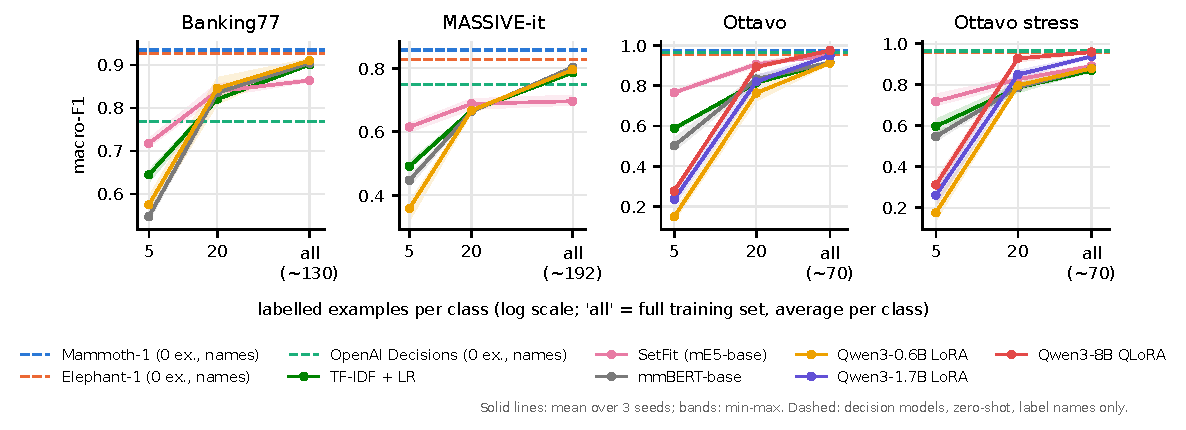
\includegraphics[width=\linewidth]{learning_curves.pdf}
\caption{Macro-F1 against labelled examples per class (log scale). Dashed: decision models used zero-shot with label names only (condition N), which uses no labelled example of the task.}
\label{fig:learning}
\end{figure}

\begin{figure}[t]
\centering
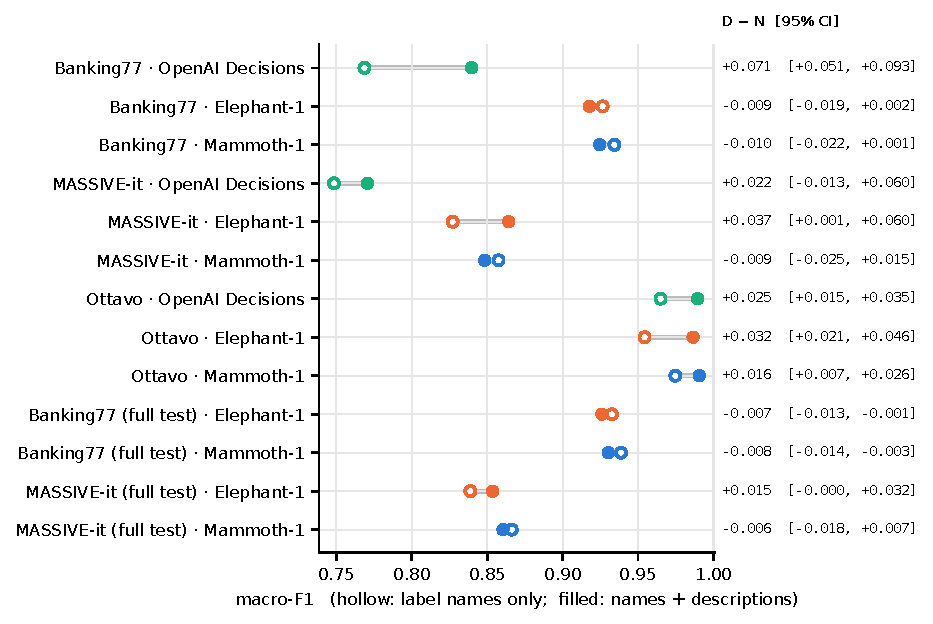
\includegraphics[width=0.62\linewidth]{descriptions_effect.pdf}
\caption{Effect of category descriptions on the same messages (N $\to$ D), with paired 95\% bootstrap intervals.}
\label{fig:descriptions}
\end{figure}

\begin{table}[t]
\centering\scriptsize
\caption{Paired contrasts other than the label-budget families (macro-F1 difference A$-$B; 95\% bootstrap interval, not adjusted for multiplicity; bootstrap $p$ Holm-adjusted within each family). P1--P5 were pre-declared; S1 was declared before its runs. Budget families P2 and P2N are in \texttt{reports/contrasts.csv}.}
\label{tab:contrasts}
\setlength{\tabcolsep}{4pt}
\begin{tabular}{lllrll}
\toprule
Data & A & B & $\Delta$ macro-F1 & 95\% CI & $p_{\mathrm{Holm}}$ \\
\midrule
\multicolumn{6}{l}{\textit{P1: descriptions, D $-$ N}} \\
Banking77 & OpenAI D & OpenAI N & +0.071 & [+0.051, +0.093] & $<$0.001 \\
Banking77 & Elephant-1 D & Elephant-1 N & -0.009 & [-0.019, +0.002] & 0.410 \\
Banking77 & Mammoth-1 D & Mammoth-1 N & -0.010 & [-0.022, +0.001] & 0.410 \\
MASSIVE-it & OpenAI D & OpenAI N & +0.022 & [-0.013, +0.060] & 0.654 \\
MASSIVE-it & Elephant-1 D & Elephant-1 N & +0.037 & [+0.001, +0.060] & 0.308 \\
MASSIVE-it & Mammoth-1 D & Mammoth-1 N & -0.009 & [-0.025, +0.015] & 0.736 \\
Ottavo & OpenAI D & OpenAI N & +0.025 & [+0.015, +0.035] & $<$0.001 \\
Ottavo & Elephant-1 D & Elephant-1 N & +0.032 & [+0.021, +0.046] & $<$0.001 \\
Ottavo & Mammoth-1 D & Mammoth-1 N & +0.016 & [+0.007, +0.026] & $<$0.001 \\
Banking77 (full test) & Elephant-1 D & Elephant-1 N & -0.007 & [-0.013, -0.001] & 0.224 \\
Banking77 (full test) & Mammoth-1 D & Mammoth-1 N & -0.008 & [-0.014, -0.003] & 0.045 \\
MASSIVE-it (full test) & Elephant-1 D & Elephant-1 N & +0.015 & [-0.000, +0.032] & 0.366 \\
MASSIVE-it (full test) & Mammoth-1 D & Mammoth-1 N & -0.006 & [-0.018, +0.007] & 0.736 \\
\midrule
\multicolumn{6}{l}{\textit{P3: progenitor}} \\
Ottavo & Elephant-1 D & Qwen3.5-9B D & +0.013 & [+0.003, +0.024] & 0.009 \\
Ottavo & Qwen3.5-9B D & Qwen3-8B D & +0.032 & [+0.018, +0.047] & $<$0.001 \\
Ottavo stress & Elephant-1 D & Qwen3.5-9B D & +0.030 & [+0.017, +0.046] & $<$0.001 \\
Ottavo stress & Qwen3.5-9B D & Qwen3-8B D & +0.067 & [+0.046, +0.093] & $<$0.001 \\
\midrule
\multicolumn{6}{l}{\textit{P4: adaptation of Qwen3-8B}} \\
Ottavo & Qwen3-8B QLoRA k=5 & Qwen3-8B D & -0.665 & [-0.688, -0.645] & $<$0.001 \\
Ottavo & Qwen3-8B QLoRA k=20 & Qwen3-8B D & -0.048 & [-0.068, -0.030] & $<$0.001 \\
Ottavo & Qwen3-8B QLoRA all data & Qwen3-8B D & +0.033 & [+0.019, +0.048] & $<$0.001 \\
Ottavo stress & Qwen3-8B QLoRA k=5 & Qwen3-8B D & -0.590 & [-0.626, -0.557] & $<$0.001 \\
Ottavo stress & Qwen3-8B QLoRA k=20 & Qwen3-8B D & +0.027 & [-0.002, +0.058] & 0.067 \\
Ottavo stress & Qwen3-8B QLoRA all data & Qwen3-8B D & +0.058 & [+0.035, +0.086] & $<$0.001 \\
\midrule
\multicolumn{6}{l}{\textit{P5: recipe (prot.: protocol recipe; expl.: exploratory recipe)}} \\
Ottavo & Qwen3-0.6B k=5 prot. & Qwen3-0.6B k=5 expl. & +0.000 & [-0.016, +0.018] & 1.000 \\
Ottavo & Qwen3-0.6B k=20 prot. & Qwen3-0.6B k=20 expl. & +0.076 & [+0.057, +0.095] & $<$0.001 \\
Ottavo & Qwen3-8B k=5 prot. & Qwen3-8B k=5 expl. & +0.004 & [-0.030, +0.036] & 1.000 \\
Ottavo & Qwen3-8B k=20 prot. & Qwen3-8B k=20 expl. & +0.022 & [+0.003, +0.042] & 0.072 \\
\midrule
\multicolumn{6}{l}{\textit{S1: recipe sensitivity, all data}} \\
Banking77 & Qwen3-0.6B expl. & Qwen3-0.6B prot. & +0.026 & [+0.018, +0.035] & $<$0.001 \\
Banking77 & Mammoth-1 D & Qwen3-0.6B expl. & -0.011 & [-0.025, +0.002] & 0.312 \\
Banking77 & Mammoth-1 N & Qwen3-0.6B expl. & -0.002 & [-0.014, +0.011] & 1.000 \\
Banking77 (full test) & Qwen3-0.6B expl. & Qwen3-0.6B prot. & +0.028 & [+0.023, +0.033] & $<$0.001 \\
Banking77 (full test) & Mammoth-1 D & Qwen3-0.6B expl. & -0.007 & [-0.014, +0.001] & 0.264 \\
Banking77 (full test) & Mammoth-1 N & Qwen3-0.6B expl. & +0.001 & [-0.006, +0.008] & 1.000 \\
\bottomrule
\end{tabular}
\end{table}

\begin{figure}[t]
\centering
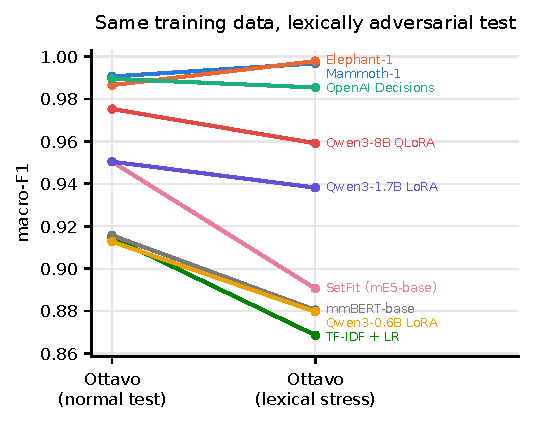
\includegraphics[width=0.48\linewidth]{stress.pdf}\hfill
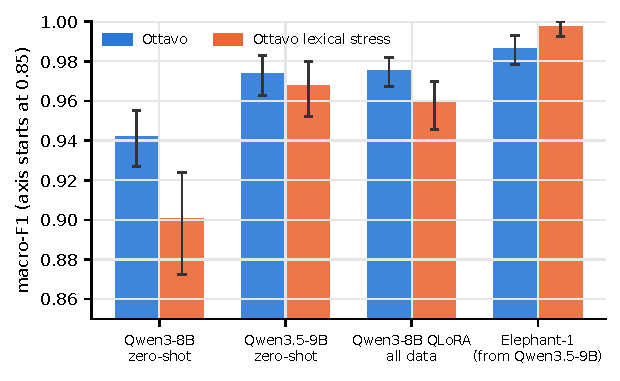
\includegraphics[width=0.48\linewidth]{progenitor.pdf}
\caption{Left: Ottavo normal vs.\ lexical stress test for the same systems. Right: generalist controls, task-adapted Qwen3-8B and
Elephant-1 on Ottavo (95\% bootstrap intervals; the axis starts at 0.85).}
\label{fig:stress}
\end{figure}

\begin{table}[t]
\centering\small
\caption{Ottavo-R test half, by phenomenon: accuracy for closed-set phenomena, clean/perturbed consistency, multi-intent prediction
among the two declared intents, and share routed to review with the threshold chosen on the dev half. Trained systems: all Ottavo training data, mean over three seeds; 5- and 20-shot rows are in \texttt{reports/robustness.csv}.}
\label{tab:robust}
\resizebox{\linewidth}{!}{\begin{tabular}{llrrrrrrrrrr}
\toprule
System & Setting & Neg. & Corr. & Distr. & Short & Typos & Cons. & Multi & Amb.$\to$rev. & OOS$\to$rev. & In-scope$\to$rev. \\
\midrule
Mammoth-1 & zero-shot, D & 1.00 & 1.00 & 1.00 & 1.00 & 1.00 & 1.00 & 0.95 & 0.56 & 0.80 & 0.30 \\
Elephant-1 & zero-shot, D & 1.00 & 1.00 & 1.00 & 1.00 & 1.00 & 1.00 & 1.00 & 0.94 & 0.80 & 0.28 \\
OpenAI Decisions & zero-shot, D & 1.00 & 1.00 & 1.00 & 1.00 & 1.00 & 1.00 & 1.00 & 0.89 & 0.90 & 0.14 \\
Qwen3-8B zero-shot & zero-shot, D & 0.95 & 0.80 & 0.95 & 1.00 & 1.00 & 1.00 & 1.00 & 0.61 & 0.90 & 0.19 \\
Qwen3.5-9B zero-shot & zero-shot, D & 1.00 & 1.00 & 0.95 & 1.00 & 1.00 & 1.00 & 0.90 & 0.83 & 0.85 & 0.28 \\
TF-IDF + LR & all Ottavo data & 0.75 & 0.80 & 0.85 & 1.00 & 1.00 & 1.00 & 0.90 & 0.72 & 1.00 & 0.17 \\
SetFit (mE5-base) & all Ottavo data & 1.00 & 0.80 & 0.75 & 0.88 & 1.00 & 1.00 & 0.97 & 0.93 & 0.55 & 0.20 \\
mmBERT-base & all Ottavo data & 0.83 & 0.70 & 0.77 & 0.93 & 0.98 & 0.97 & 0.93 & 0.83 & 0.70 & 0.34 \\
Qwen3-0.6B LoRA & all Ottavo data & 0.93 & 0.82 & 0.77 & 0.82 & 0.98 & 0.97 & 0.97 & 0.83 & 0.67 & 0.23 \\
Qwen3-1.7B LoRA & all Ottavo data & 1.00 & 0.80 & 0.92 & 0.92 & 1.00 & 1.00 & 0.97 & 0.83 & 0.70 & 0.19 \\
Qwen3-8B QLoRA & all Ottavo data & 0.97 & 0.93 & 0.98 & 0.93 & 1.00 & 1.00 & 0.97 & 0.78 & 0.85 & 0.18 \\
\bottomrule
\end{tabular}}
\end{table}
